%! Author = Adrian Helberg
%! Date = 20.10.2020

% Preamble
\documentclass[12pt]{beamer}
\usetheme{Marburg}
\usepackage{ngerman}
\usepackage{graphicx}

\title{Arbeitspakete}
\author{Adrian Helberg}
\date{\today}

% Document
\begin{document}
    \maketitle

    \section{Arbeitspaket 1}
    \begin{frame}
        \frametitle{Beschreibung}
        In Arbeitspaket 1 soll die grafische Benutzeroberfläche erstellt werden. Es umfasst die
        Bereiche:
        \begin{itemize}
            \item[I.] Strukturieren
            \item[II.] Visualisieren
        \end{itemize}
        \\~\\
        \textit{siehe Exposé Kapitel 1.1.2 Überblick}
    \end{frame}

    \begin{frame}[fragile]
        \frametitle{Ablauf}
        Das Programm soll folgenden Workflow umsetzen:\\~\\
        \begin{itemize}
            \item[1] Erster Anker ist vorselektiert
            \item[2] Widerhole, bis Struktur erstellt ist:
            \begin{itemize}
                \item[2.1] Selektiere ein Template aus der Liste
                \item[2.2] Setze Parameter
                \item[2.3] Bestätige Auswahl und Parameter
                \item[2.4] Zeichne ausgewähltes Template mit Parametern
                \item[2.5] Wähle nächsten Anker aus
            \end{itemize}
        \end{itemize}
    \end{frame}

    \begin{frame}
        \frametitle{Layout}
        \begin{figure}
            \centering
            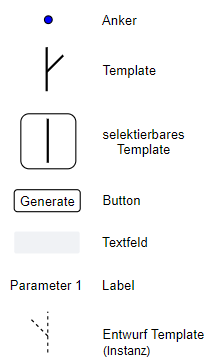
\includegraphics[width=3cm]{../images/UI_Legende.PNG}
            \caption{Legende}
        \end{figure}
    \end{frame}

    \begin{frame}
        \frametitle{Beispiel}
        \begin{figure}
            \centering
            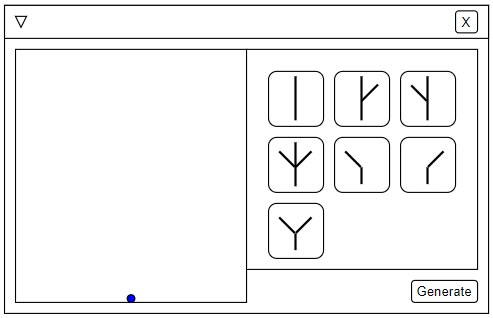
\includegraphics[width=4cm]{../images/UI_1.PNG}
            \caption{Erster Anker ist vorselektiert}
        \end{figure}
        \begin{figure}
            \centering
            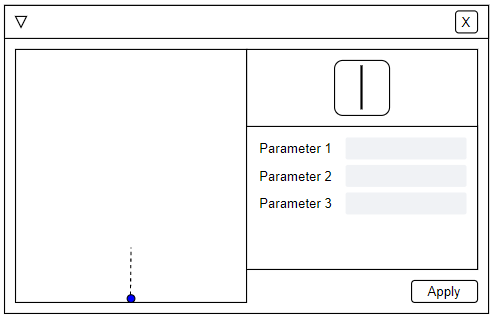
\includegraphics[width=4cm]{../images/UI_2.PNG}
            \caption{Setze Parameter (1/2)}
        \end{figure}
    \end{frame}

    \begin{frame}
        \frametitle{Beispiel}
        \begin{figure}
            \centering
            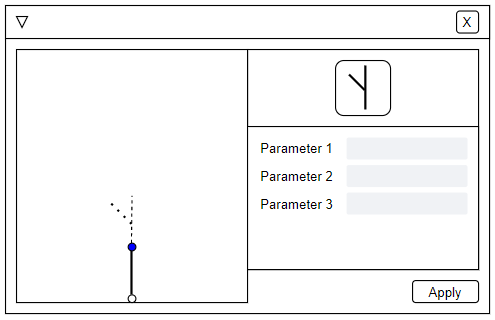
\includegraphics[width=4cm]{../images/UI_4.PNG}
            \caption{Setze Parameter (2/2)}
        \end{figure}
        \begin{figure}
            \centering
            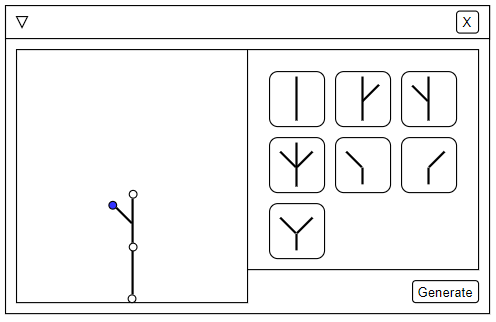
\includegraphics[width=4cm]{../images/UI_5.PNG}
            \caption{Zeichne Template nach Bestätigung (\textit{apply})}
        \end{figure}
    \end{frame}

    \begin{frame}
        \frametitle{Beispiel}
        \begin{figure}
            \centering
            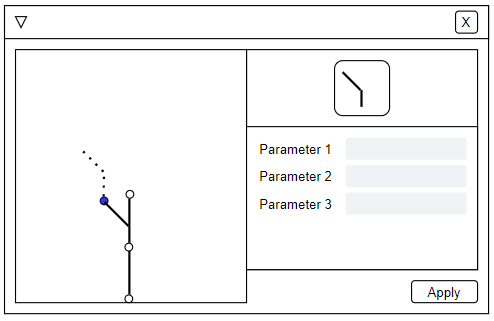
\includegraphics[width=4cm]{../images/UI_6.PNG}
            \caption{Selektierter Anker 1}
        \end{figure}
        \begin{figure}
            \centering
            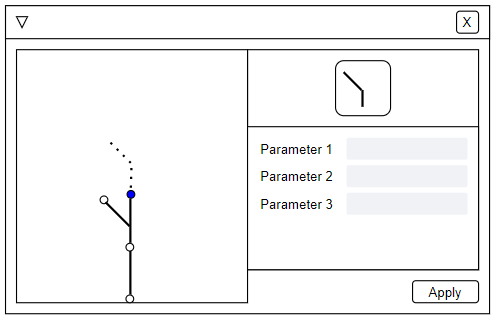
\includegraphics[width=4cm]{../images/UI_7.PNG}
            \caption{Selektierter Anker 2}
        \end{figure}
    \end{frame}

    \section{Arbeitspaket 2}
    \begin{frame}
        \frametitle{Beschreibung}
        In Arbeitspaket 2 soll die Baumstruktur aufgebaut werden
    \end{frame}

    \section{Arbeitspaket 3}
    \begin{frame}
        \frametitle{Beschreibung}
        Arbeitspaket 3
    \end{frame}

    \section{Arbeitspaket 4}
    \begin{frame}
        \frametitle{Beschreibung}
        Arbeitspaket 4
    \end{frame}

\end{document}